\section{Game development}
In this section, the different components of video game development and how it differs from ordinary application development are analysed. Afterwards, some examples of tools for game development are described, namely \textit{Scratch}, GameMaker and PyGame. This is done to develop a better understanding of which kinds of tools are available to a new developer.

%This section will analyse how games are developed right now, how flow of the project is when you program the game and how this flow can different then a more normal project flow, in a company where you have to make program to some one. after this there will be a look at some of the tools that exist to make this easy for people to program like block programing, here should be look at scratch, then there are combination of block and text programing, here should be look at GameMaker since this still have block program but also text base program in the languge GML(GameMaker Language) and at last only text base programing in this case here should be looked at PyGame this is in python and is a layer over SDL that give easy access to some thing that you need in game develoment.

\subsection{Components of game development}
%To better understand how game development differs from more conventional development, it is important to first understand how to develop a video games.


To develop a video game, the developer needs to manage components that are specific for the domain of game development. All video games must be able to handle user input and have a way to display some sort of output to the user. This output is often in the form of graphics drawn by the graphics card to the screen. Depending on the kind of video game that is being developed, different components are needed. These components include, but are not limited to: 

\begin{itemize}
 \item Collision Detection
 \item Physics
 \item Animation
 \item Graphics (2D and 3D)
 \item Artificial Intelligence
 \item User Input
 \item File Input/Output
 \item Networking \ldots
\end{itemize}

%When developers work on a game they work close together with a team of game designers in bigger companies, they stand for the vision of the game, how they think it should what could be fun the sound the image models and all of those tings you job as the game programmer is to take there's vision and turn it in to realty on the hardware and software you have. and this can be very hard since there so many components in the development of a game, a few things you need to make.\cite{DesignVSPrograming2016}

There are different tools and frameworks that add abstraction layers to game development so that a developer can focus on developing a game, instead of having to spend a lot of time on implementing things like graphics, physics and networking. Some of these tools are described in the following section.

%many of those things can be made easy to understand and use in a program language that is design to make games in, and this will give a faster and better work, and can help introducing new people the programing and game development.

%To answer the question "How is the flow of game development different than programming a normal piece of software?",  \cite{StackGameVSSoftware2011} on a forum post there have been a few people that did talk about their experience in the field of gaming, and how they think it is different, one say that the different lay in the size of the project and a bigger risk and other say that it is the target of what you try to do, when you make a program for a company, you need to make it easy to use and have all the features that ask for, but in the game you need besiege the easy of use also that it is fun to use/play, and that have to think about this under the hole project is he say was the hardes part, and they there where those that say that there were no real different between the two that it was the same thing, so like with software you make for other company's it is something that chance from project to project and is never the same.



\subsection{Existing solutions}
There is a number of tools to develop video games. To best understand the domain, three different tools are described in the following section, namely \textit{Scratch}, \textit{GameMaker} and \textit{PyGame}.
These have been chosen, since they each represent a different approach to video game development.

%In this subsection, three different existing tools with three different approaches are described. The first solution uses block programming only, the second uses both block programming and textual programming, and the third uses textual programming only. This way, \todo{pls help}

\subsubsection{Scratch}
Scratch is a visual programming language, which means that the user programs with a graphical interface rather than a textual one. It utilises block programming instead of actual code. This way, the user does not learn to write code, but rather the mindset of programming. The blocks are conveniently grouped in relevant groups. For example, the group "motion" contains the "move" block, which makes the character move a certain amount of steps, and "turn" blocks, which makes the character turn either clockwise or counterclockwise. By putting these kinds of blocks together, Scratch translates it to actual code.

\begin{figure}[H]
\centering
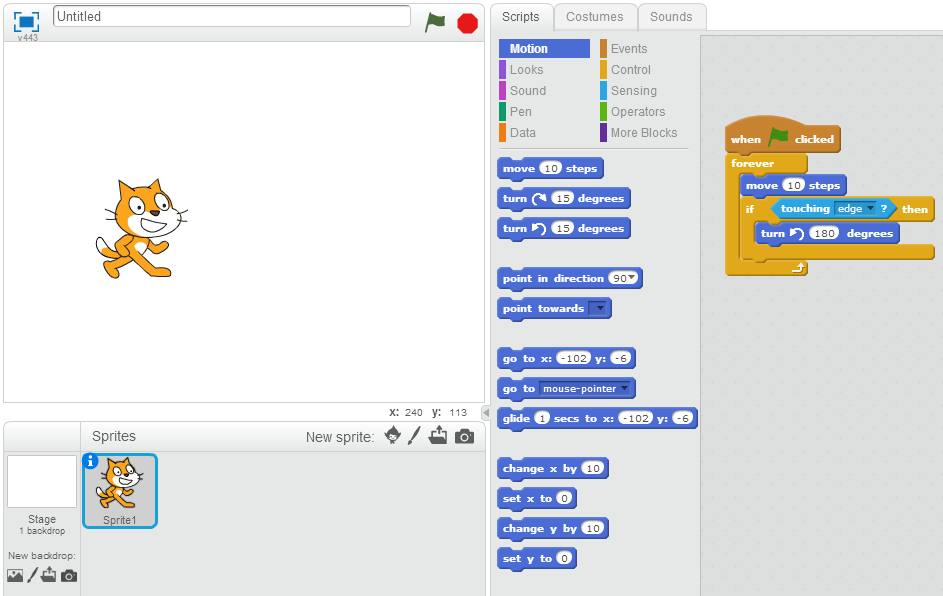
\includegraphics[scale=0.5]{resources/Images/Scratch.png}
\caption{Small program made in Scratch}
\label{fig:Scratch}
\end{figure}

On figure \ref{fig:Scratch} a simple program made in Scratch is seen. This program makes the character indefinitely walk 10 steps in one direction and rotate the character 180 degrees if it hits the wall. The green flag corresponds to running the main function of a conventional programming language.
The easy-to-learn interface and the child friendly design, makes Scratch an ideal solution for the youngest people who wants to be introduced to the world of programming.\cite{scratch}

\subsubsection{GameMaker}
GameMaker is a game making software that implements a mixture of drag and drop programming and their own language called GameMaker Language, which is an interpreted scripting language based on C. This way, it is possible to create games quickly and easily with the drag and drop while at the same time having flexibility and control of conventional programming with GameMaker Language.

\begin{figure}[H]
\centering
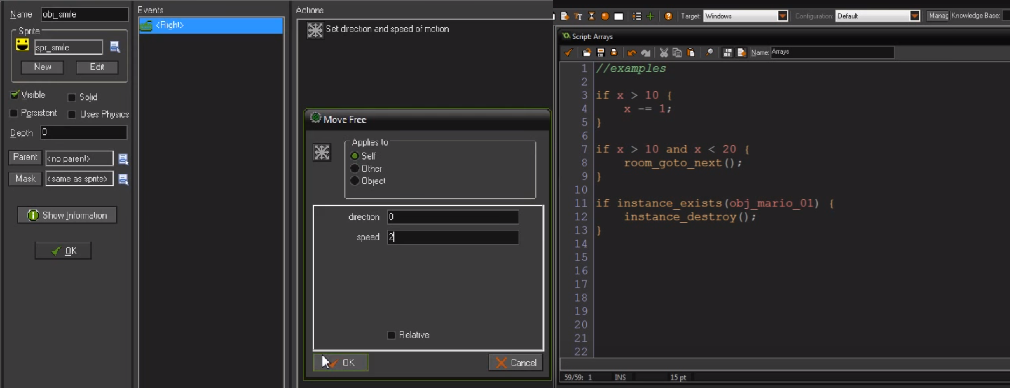
\includegraphics[scale=0.5]{resources/Images/GameMaker.PNG}
\caption{On the left is drag and drop\cite{GMDnD}. On the right is GML \cite{GML}}
\label{fig:GameMaker}
\end{figure}

On figure \ref{fig:GameMaker} an example of the two is shown. On the left is the drag and drop system, where actions gets paired with events. In this example, the right arrow key makes obj\_smile move 2 pixels per frame towards direction 0. On the right side, examples of if-statements in GML are pictured.

\subsubsection{PyGame}
PyGame is a set of Python modules used to make it easier to make games in the programming language Python. This means that it adds a number of functionalities which aid in the game making process. PyGame utilises fully conventional coding and requires the programmer to write actual code.
An example of functionalities is pygame.event.get(), which retrieves every event currently in queue to get handled.

\begin{figure}[H]
\centering
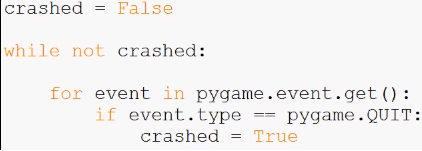
\includegraphics[scale=0.6]{resources/Images/PyGame.png}
\caption{Small PyGame program}
\label{fig:PyGame}
\end{figure}

Figure \ref{fig:PyGame} uses this functionality by checking every event in the queue. Furthermore, it uses pygame.QUIT which is the event type in PyGame that means that the close button has been pressed. Therefore, this code checks every event in the queue if they are a click on the close button. If they are, the program breaks out of the for loop.

\subsection{Target audience}
\label{sub:TargetAudience}
The tools described in this chapter cover a wide spectrum in terms of beginner friendly game development. Scratch\cite{scratch} is easy to use for beginners, and Pygame is meant for more experienced developers. There is, however, a slot somewhere in between Scratch and GameMaker/Pygame, which has to help beginners going from scratch to something like Pygame, and introduce them to control structures, boolean logic, and other concepts of programming. This transition could turn some off from wanting to do more programming, as it may seem too complicated and scary. This is why there is a need for a language in between these two types of programming languages that is simple and easy to learn. Furthermore Scratch looks and feels child-friendly, which is not appealing for a teenager, who wants to be introduced to some less basic concepts of programming while at the same time not getting a lot of advanced and confusing features.

For a textual programming language to have any functionality, it has to use mathematics. These include vectors used in, among others, simulating motion of objects and basic algebra used in variables, which are very essential parts of game development.
As these are an essential part of programming, the target audience has to know, or at least have the preliminary knowledge needed to learn these concepts. As seen in \cite{FFMM} from the Ministry of education, students are introduced to use variables from around the sixth grade in Denmark, but will not learn to use functions and equations before seventh to ninth grade. Therefore, the target audience (TA) is chosen to be students starting from the ninth grade.



With this in mind, there will in the following section be defined a problem statement.